% !TEX TS-program = lualatex

\documentclass[14pt,russian,a4paper]{extreport}
 
\input{../preamble_bmstu_lua.tex}

\usepackage{geometry}
\geometry{left=3cm}
\geometry{right=2cm}
\geometry{top=2cm}
\geometry{bottom=2.2cm}

\addbibresource{biblio.bib}

\usepackage{tikz}
\newcommand*\circled[1]{\tikz[baseline=(char.base)]{
             \node[shape=circle,draw,inner sep=2pt, minimum size=8mm] (char) {#1};}}

\cfoot{}
\rfoot{\thepage}
\fancypagestyle{plain}{ 
    \fancyhf{}
    \cfoot{}
    \rfoot{\thepage}}


\linespread{1.4} % полуторный интервал
\frenchspacing

\setcounter{tocdepth}{1}

\titleformat{\chapter}
    {\filcenter\normalsize\bfseries}{\thechapter}{0.7em}
    {\trackedcaps}

\faculty{М-КФ «Машиностроительный»}
\department{М1-КФ «Машиностроительные технологии»}
\reportname{Курсовой проект}
\discipline{Основы конструирования приспособлений}
\thetopic{Проектирование станочных приспособлений}
\writtenby{студент группы ТМД.Б-71 Куркин М. В.}
\checkedby{Попков В. М.}
\thefooter{Калуга, 2018 г.}

\begin{document}

\input{../title_bmstu_dz.tex}

\setcounter{page}{3}

\tableofcontents

\chapter{Анализ исходных данных}

\section{Cлужебное назначение детали}

Обрабатываемая деталь --- корпус барабана. Детали типа «корпус» предназначены для крепления к ним других деталей и сборочных единиц изделия. Корпусные детали обеспечивают точность и постоянство относительного расположения прикрепляемых к ней деталей, поэтому должны обладать достаточной жёсткостью. Обрабатываемая деталь является вращающейся.\par

Наружная поверхность детали --- призма, основанием которой является правильный шестиугольник с диаметром вписанной окружности $\SI{620}{\milli\meter}$. С обеих торцов призмы деталь имеет ряд выступов, образующих цилиндрические и конические поверхности. На каждой грани шестигранника расположено по четыре штифтовых отверстия $\SI{20}[\diameter]{H7 \; \milli\meter}$ и по восемь резьбовых M12. \par

Ступица детали имеет отверстие $\SI{125}[\diameter]{H7 \; \milli\meter}$, предназначенное для ус\-тановки детали на вал. На внешней части ступицы расположен паз. Ступица соединена с наружной частью детали полотном. На нём расположены 6 рёбер, служащих для повышения жёсткости детали. В перемычках между спицами выполнены два такеллажных отверстия $\SI{100}[\diameter]{\milli\meter}$.  \par

Кроме перечисленных, деталь имеет ряд резьбовых и штифтовых отверстий, необходимых для прикрепления к корпусу других деталей изделия. \par

Заготовка детали --- отливка из серого чугуна СЧ~21-40 (ГОСТ~1412-85). \par



\section{Анализ технических условий на изготовление~детали}

Наиболее точные цилиндрические поверхности детали --- отверстие в ступице $\SI{125}[\diameter]{H7 \; \milli\meter}$, 6 отверстий $\SI{45}[\diameter]{H7 \; \milli\meter}$, 2 отверстия $\SI{25}[\diameter]{H7 \; \milli\meter}$, 26 отверстий $\SI{20}[\diameter]{H7 \; \milli\meter}$ и 6 отверстий $\SI{12}[\diameter]{H7 \; \milli\meter}$. Необходимость их высокой точности обусловлена тем, они являются сопрягаемыми. Для менее точных поверхностей заданы их предельные отклонения: $\SI{600}[\diameter]{_{-0,2} \; \milli\meter}$ и $\SI{590}[\diameter]{_{-0,5} \; \milli\meter}$. Заданные предельные отклонения удовлетворяют требованиям, соответственно, 10 и 12 квалитетов. Размеры с неуказанными предельными отклонениями выполняются по 14 квалитету. \par

Точность взаимного расположения поверхностей детали задана допусками параллельности торцовых поверхностей детали относительно друг друга и перпендикулярности наружных граней корпуса относительно торца, которые составляют $\SI{0,03}{\milli\meter}$, и допуском радиального биения наружной цилиндрической поверхности $\SI{600}[\diameter]{_{-0,2} \; \milli\meter}$ относительно посадочного отверстия ступицы $\SI{125}[\diameter]{H7 \; \milli\meter}$, который составляет $\SI{0,1}{\milli\meter}$. \par

Точность формы задана допусками на плоскостность торца и наружных граней корпуса, который составляет $\SI{0,02}{\milli\meter}$. \par

Шероховатость задана значениями Ra~1,25 для посадочного отверстия ступицы $\SI{125}[\diameter]{H7 \; \milli\meter}$ и других сопрягаемых отверстий, Ra~2,5 для плоскоских поверхностей наружных граней и торцов корпуса и для внутренней цилиндрической поверхности $\SI{430}[\diameter]{\milli\meter}$, и Ra~10 для плоских поверхностей торцов ступицы, наружных цилиндрических поверхностей $\SI{590}[\diameter]{_{-0,5} \; \milli\meter}$ и отдельных резьбовых отверстий. Для остальных поверхностей задана шероховатость Rz~630, получаемая без применения механической обработки.


\section{Характеристика материала заготовки}

Материал заготовки --- серый чугун СЧ~21-40 (ГОСТ~1412--85). Это чугун с пластинчатым графитом для отливок с временным сопротивлением при растяжении не менее $\sigma_B = \SI{210}{\mega\pascal}$. \par

Серый чугун --- сравнительно дешёвый конструкционный материал. Имеет хорошие литейные и технологические свойства. Из серого чугуна изготавливают массивные литые детали, такие как станины, маховики, крупногабаритные корпуса. \par

Физические свойства чугуна СЧ~21-40: плотность $\rho = \SI{7100}{\kilo\gram\per\meter\cubed}$, линейная усадка $\varepsilon = \SI{1,2}{\percent}$, модуль упругости при растяжении $E = \SIrange[allow-number-unit-breaks]{850}{1100e-5}{\mega\pascal}$, удельная теплоёмкость при $t = \SIrange{20}{200}{\celsius}$ $c = \SI{480}{\joule\per\kilo\gram\per\kelvin}$, коэффициент линейного расширения при $t = \SIrange{20}{200}{\celsius}$ $\alpha = \SI[per-mode=reciprocal]{9,5e-6}{\per\celsius}$, теплопроводность при $\SI{20}{\celsius}$ $\lambda = \SI{54}{\watt\per\meter\per\kelvin}$. \par

Химический состав чугуна СЧ~21-40: массовая доля углерода $\SIrange{3,3}{3,5}{\percent}$, кремния --- $\SIrange{1,4}{2,4}{\percent}$, марганца --- $\SIrange{0,7}{1,0}{\percent}$, фосфора --- не более $\SI{0,2}{\percent}$, серы --- не более $\SI{1,5}{\percent}$. Допускается низкое легирование чугуна различными элементами (хромом, никелем, медью, фосфором и другими).


\section{Анализ технологичнсти конструкции детали}

Большинство конструктивных элементов детали унифицированы. 

Точность размеров и шероховатость поверхностей экономически и конструктивно обоснованы. 

Физико-химические и механические свойства материала, жёсткость детали, её форма и размеры соответствуют требованиям технологии изготовления, конструкция жёсткая.

Деталь имеет технологические базы, позволяющие обеспечить точность установки, обработки и контроля.

Обработка и контроль точных поверхностей детали не затруднены.

Деталь имеет большое количество глухих точных отверстий, что усложняет обработку.

Шпоночный паз расположен нетехнологично, его обработка затрудняется необходимостью располагать деталь под углом.

Большая масса и габаритные размеры заготовки усложняют транспортировку и установку детали на станке.

Конструкция детали в целом технологична, но имеет ряд элементов, обработка которых затруднена.


\chapter{Проектирование операций механической обработки детали}

\section{Проектирование сверлильной операции с ЧПУ}

\subsection{Выбор и характеристика оборудования}
Операция выполняется на горизонтальном сверлильно\-/фрезерно\-/расточном станке с ЧПУ и АСИ 2206ВМФ4. 

Это станок с крестовым поворотным столом, предназначенный для комплексной обработки плоских деталей средних размеров сложной формы. Станок предназначен дял многооперационной обработки разнообразных деталей сложной конфигурации из стали, чугуна, цветных и лёгких сплавов. На станке можно производить получистовое и чистовое фрезерование плоскостей, пазов и криволинейных поверхностей различными типами фрез, а также растачивание, сверление, зенкерование, развёртывание отверстий и нарезание резьбы метчиками и резцами по заданной программе. Станок может быть использован в мелкосерийном и серийном производствах различных отраслей промышленности.

Управление станком --- от универсальной комплексной системы ЧПУ «Размер-2М-1300», позволяющей производить позиционную и контурную обработку, а также вручную с пульта управления. На станке программируются координатные перемещения стола и шпиндельной головки, скорости этих перемещений, частота вращения шпинделя, выбор и смена инструмента, смена обрабатываемой детали и циклы обработки.

На станке программируются координатные перемещения стола, шпиндельной головки, скорости этих перемещений, режимы обработки, выбор, смена и коррекция инструмента, циклы обработки.

Станок может быть оснащен устройством автоматической загрузки и выгрузки изделий, предназначенным для установки заготовки вне станка на сменные столы (паллеты) и последующей автоматической загрузки столов на станок, а также их выгрузки со станка после окончания обработки. Использование сменных столов устройства позволяет совместить загрузку заготовок или выгрузку обработанных изделий с работой станка, что существенно сокращает холостые простои, повышает эффективность его использования и производительность, при этом исключается последняя ручная операция --- установка и снятие деталей со станка.

Основные характеристики станка:
\begin{itemize}
  \item Класс точности станка В по ГОСТ 8-82
	\item Размеры рабочей поверхности стола $\SI{630 x 800}{\milli\meter}$
  \item Расстояние от торца шпинделя до центра стола $\SIrange{195}{825}{\milli\meter}$
	\item Наибольшее продольное перемещение стола (X) $\SI{800}{\milli\meter}$
	\item Наибольшее поперечное перемещение стола (Z) $\SI{630}{\milli\meter}$
	\item Наибольшее вертикальное перемещение шпиндельной головки (Y) $\SI{630}{\milli\meter}$
	\item Наибольшая нагрузка на стол $\SI{800}{\kilo\gram}$
	\item Ёмкость инструментального магазина $\SI{30}{\pcs}$
	\item Наибольший диаметр устанавливаемого инструмента $\SI{200}{\milli\meter}$
	\item Наибольшая длина инструмента, устанавливаемого в шпинделе станка $\SI{400}{\milli\meter}$
	\item Частота вращения шпинделя $\SIrange{10}{3500}{\rev\per\minute}$
	\item Электродвигатель привода шпинделя $\SI{15}{\kilo\watt}$
	\item Масса станка $\SI{12}{\tonne}$
\end{itemize}

\newpage
На рис.~\ref{fig:2206} приведены габариты рабочего пространства сверлильно\-/фрезерно\-/расточного станка 2206ВМФ4 (\subref{subfig:2206a}) и его посадочные и присоединительные размеры (\subref{subfig:2206b}, \subref{subfig:2206c}, \subref{subfig:2206d}).

\begin{figure}[H]
	\centering
  \begin{subfigure}[b]{.50\textwidth}
    \centering
    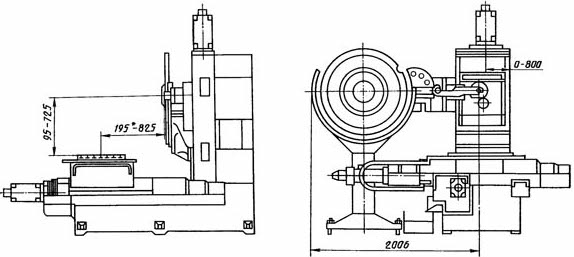
\includegraphics[width=.90\linewidth]{spr_2206vmf4_1.jpg}
    \caption{габаритные размеры рабочего поля}
    \label{subfig:2206a}
  \end{subfigure}%
  \begin{subfigure}[b]{.50\textwidth}
    \centering
    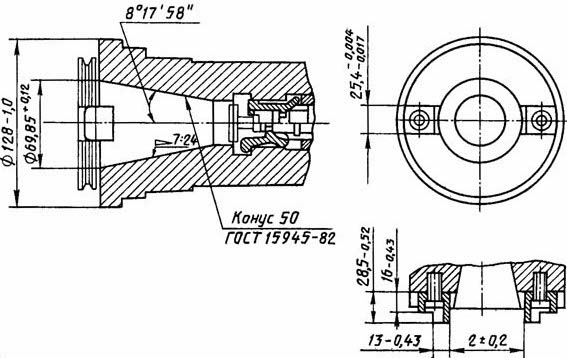
\includegraphics[width=.90\linewidth]{spr_2206vmf4_2.jpg}
    \caption{посадочные и присоединительные базы}
    \label{subfig:2206b}
  \end{subfigure} \\
  \begin{subfigure}[b]{.50\textwidth}
    \centering
    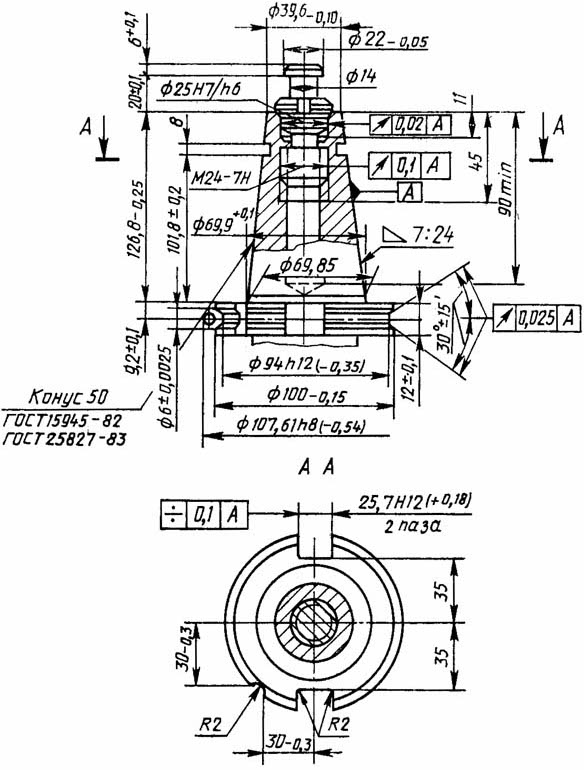
\includegraphics[width=.90\linewidth]{spr_2206vmf4_3.jpg}
    \caption{конец инструмента}
    \label{subfig:2206c}
  \end{subfigure}%
  \begin{subfigure}[b]{.50\textwidth}
    \centering
    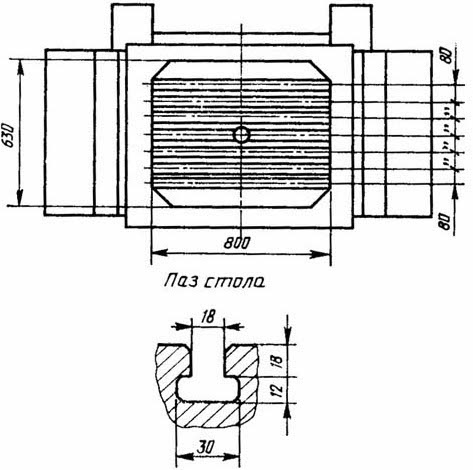
\includegraphics[width=.90\linewidth]{spr_2206vmf4_4.jpg}
    \caption{рабочий стол}
    \label{subfig:2206d}
  \end{subfigure}%
  \caption{Посадочные и присоединительные размеры станка 2206ВМФ4}
  \label{fig:2206}
\end{figure}

\newpage
\subsection{Выбор и обоснование схемы базирования}

Базирование осуществляется по схеме, представленной на рис.~\ref{fig:b040}

\begin{figure}[H]
	\centering
	   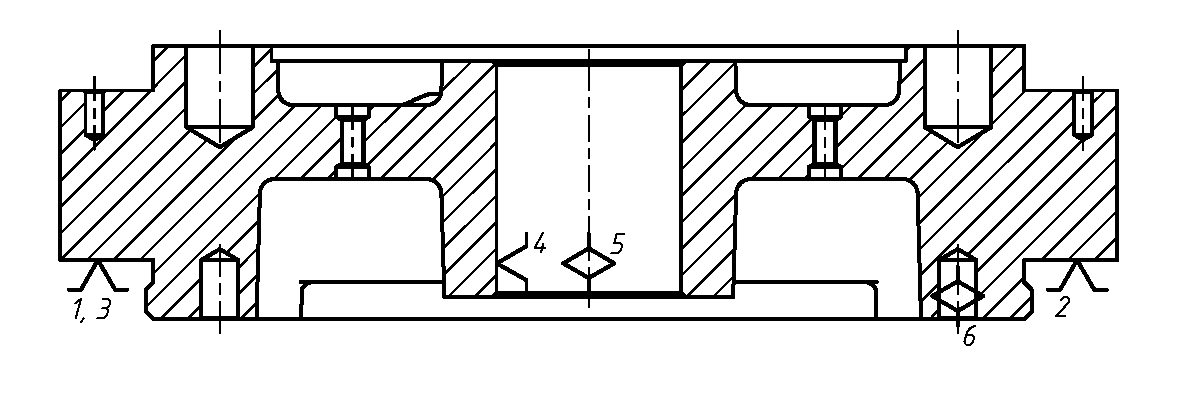
\includegraphics[width=0.7\textwidth]{bases_040.pdf}
	   \caption{Схема базирования на операции 040}
	   \label{fig:b040}
	   1, 2, 3 --- установочная база, \\
	   4, 5 --- направляющая база, \\
	   6 --- опорная база
\end{figure}

\subsection{Выбор и обоснование последовательности и содержания переходов}

На операции 040 осуществляется обработка отверстий, расположенных на гранях наружной поверхности детали. Деталь установлена в специальном приспособлении, поворот относительно своей оси она осуществляет за счёт делительного движения, совершаемого поворотным столом станка. На каждой позиции последовательно обрабатываются все отверстия, расположенные на грани, обращённой к шпинделю. Обработка 4 отверстий $\SI{20}[\diameter]{H7 \; \milli\meter}$ осуществляется за три перехода последовательным сверлением, зенкерованием и развёртыванием. Обработка 8 резьбовых отверстий M12-7H производится сверлением и нарезанием резьбы метчиком. Последним переходом снимаются фаски на всех отверстиях. После этого стол станка поворачивается и обрабатывается следующая грань детали. Последовательность обработки отверстий на каждой грани приведена в табл.~\ref{tab:040}

\begin{table}[H]
  \setlength{\tabulinesep}{1.2ex}
  \begin{longtabu} to \textwidth { | X[7,l,p] | }
    \caption{Содержание основных переходов операции 040} \label{tab:040} \\
  
      \hline 
      \multicolumn{1}{|c|}{\linespread{1.1} \bfseries{\small Содержание переходов}} \\ \hline 
    \endfirsthead
  
      \multicolumn{1}{l}{{\itshape Продолжение таблицы \thetable{}}} \\ \hline 
      \multicolumn{1}{|c|}{\linespread{1.1} \bfseries{\small Содержание переходов}} \\ \hline
    \endhead
  
      \hline
    \endfoot
  
    По программе: \\
      -- Сверлить 4 отверстия \circled{35} $\diameter 18,5 \, ^{+0,130}$ на глубину $35$    \\
      -- Сверлить 8 отверстий \circled{37} $\diameter 10,2 \, ^{+0,36}$ на глубину $25$    \\
      -- Зенкеровать 4 отверстия \circled{35} $\diameter 19,7 \, ^{+0,052}$ на глубину $35$ \\
      -- Развернуть 4 отверстия \circled{35} $\diameter 20 \, ^{+0,025}$ на глубину $35$    \\
      -- Нарезать резьбу \circled{39} в 8 отверстиях М12-7H на глубину $20$	                                   \\
      -- Зенковать 12 фасок \circled{36} и \circled{38}, выдерживая размер $1,6 \times \ang{45}$ \\

      \hline

  \end{longtabu}
\end{table}

\subsection{Выбор и характеристика режущего инструмента}

Для сверления отверстий \circled{35} выбрано сверло $\diameter 18,5$ 2301-3619 ГОСТ 10903-77. Для сверления отверстий под резьбу \circled{37} выбрано сверло $\diameter 10,2$ 2301-4204 ГОСТ 22736-77. Для зенкерования отверстий \circled{35} выбран зенкер $\diameter 19,7$ 2320-0529 ГОСТ 12489-71. Для развёртывания отверстий \circled{35} выбрана развёртка $\diameter 20$ 2363-3463 ГОСТ 1672-80. Для нарезания резьбы \circled{39} выбран метчик M12 2621-1515 ГОСТ 3266-81. Для зенковки фасок \circled{36} и \circled{38} выбрана зенковка 2353-0123 ГОСТ 14953-80. 

Материал режущей части всех инструментов --- быстрорежущая сталь Р6М5~\cite[прил.~2]{guzeev:rr}.

\newpage
\subsection{Расчёт режимов и сил резания}

\subparagraph{T01} Сверление $\diameter 18,5$ \

$$ S_o = {S_o}_\text{т} K_{S_\text{м}} $$

$ {S_o}_\text{т} = \SI{0,56}{\milli\meter\per\rev} $ \cite[карта 46]{guzeev:rr} \par
$ K_{S_\text{м}} = 1,0 $ \cite[карта 53]{guzeev:rr}

$$ V = V_\text{т} K_{V_\text{м}} K_{V_\text{з}} K_{V_\text{ж}} K_{V_\text{т}} K_{V_\text{w}} K_{V_\text{и}} K_{V_\text{l}} K_{V_\text{п}} $$ 

$ V_\text{т} = \SI{22,8}{\meter\per\minute} $ \cite[карта 46]{guzeev:rr} \par
$ K_{V_\text{м}} = K_{V_\text{з}} = K_{V_\text{ж}} = K_{V_\text{т}} = K_{V_\text{w}} = K_{V_\text{и}} = K_{V_\text{l}} = K_{V_\text{п}} = 1,0 $ \cite[карта 53]{guzeev:rr} 

\begin{gather*}
  S_o = 0,56 \cdot 1,0 = \SI{0,56}{\milli\meter\per\rev} \\
  V = 22,8 \cdot 1,0 = \SI{22,8}{\meter\per\minute} \\
  n = \frac{1000 V}{\pi D} = \frac{1000 \cdot 22,8}{\pi \cdot 18,5} = \SI{392,3}{\rev\per\minute} \\
  V_s = S_o n = 0,56 \cdot 392,3 = \SI{219,7}{\milli\meter\per\minute}
\end{gather*}

Станок позволяет регулировать обороты шпинделя и подачи бесступенчато. Фактические режимы резания округляют до значений из стандартных рядов предпочтительных чисел в меньшую сторону: $n_\text{ф} = \SI{355}{\rev\per\minute}, S_o = \SI{0,56}{\milli\meter\per\rev}$; тогда ${V_S}_\text{ф} = \SI{198,8}{\milli\meter\per\minute}$. Фактическая скорость резания:

$$ V_\text{ф} = \frac{\pi D n}{1000} = \frac{\pi \cdot 18,5 \cdot 355}{1000} = \SI{20,6}{\meter\per\minute} $$

$$ N = \frac{N_\text{т}}{K_{N_\text{м}}} $$

$ N_\text{t} = \SI{2,74}{\kilo\watt} $ \cite[карта 46]{guzeev:rr} \par
$ K_{N_\text{м}} = 1,0 $ \cite[карта 53]{guzeev:rr}

$$ N = \frac{2,74}{1,0} = \SI{2,74}{\kilo\watt} $$

$$ P = \frac{P_\text{т}}{K_{P_\text{м}}} $$

$ P_\text{t} = \SI{8087}{\newton} $ \cite[карта 46]{guzeev:rr} \par
$ K_{P_\text{м}} = 1,0 $ \cite[карта 53]{guzeev:rr}

$$ P = \frac{8087}{1,0} = \SI{8087}{\newton} $$

\subparagraph{T02} Сверление $\diameter 10,2$ \

$$ S_o = {S_o}_\text{т} K_{S_\text{м}} $$

$ {S_o}_\text{т} = \SI{0,56}{\milli\meter\per\rev} $ \cite[карта 46]{guzeev:rr} \par
$ K_{S_\text{м}} = 1,0 $ \cite[карта 53]{guzeev:rr}

$$ V = V_\text{т} K_{V_\text{м}} K_{V_\text{з}} K_{V_\text{ж}} K_{V_\text{т}} K_{V_\text{w}} K_{V_\text{и}} K_{V_\text{l}} K_{V_\text{п}} $$ 

$ V_\text{т} = \SI{22,8}{\meter\per\minute} $ \cite[карта 46]{guzeev:rr} \par
$ K_{V_\text{м}} = K_{V_\text{з}} = K_{V_\text{ж}} = K_{V_\text{т}} = K_{V_\text{w}} = K_{V_\text{и}} = K_{V_\text{l}} = K_{V_\text{п}} = 1,0 $ \cite[карта 53]{guzeev:rr} 

\begin{gather*}
  S_o = 0,56 \cdot 1,0 = \SI{0,56}{\milli\meter\per\rev} \\
  V = 22,8 \cdot 1,0 = \SI{22,8}{\meter\per\minute} \\
  n = \frac{1000 V}{\pi D} = \frac{1000 \cdot 22,8}{\pi \cdot 18,5} = \SI{392,3}{\rev\per\minute} \\
  V_s = S_o n = 0,56 \cdot 392,3 = \SI{219,7}{\milli\meter\per\minute}
\end{gather*}

Станок позволяет регулировать обороты шпинделя и подачи бесступенчато. Фактические режимы резания округляют до значений из стандартных рядов предпочтительных чисел в меньшую сторону: $n_\text{ф} = \SI{355}{\rev\per\minute}, S_o = \SI{0,56}{\milli\meter\per\rev}$; тогда ${V_S}_\text{ф} = \SI{198,8}{\milli\meter\per\minute}$. Фактическая скорость резания:

$$ V_\text{ф} = \frac{\pi D n}{1000} = \frac{\pi \cdot 18,5 \cdot 355}{1000} = \SI{20,6}{\meter\per\minute} $$

$$ N = \frac{N_\text{т}}{K_{N_\text{м}}} $$

$ N_\text{t} = \SI{2,74}{\kilo\watt} $ \cite[карта 46]{guzeev:rr} \par
$ K_{N_\text{м}} = 1,0 $ \cite[карта 53]{guzeev:rr}

$$ N = \frac{2,74}{1,0} = \SI{2,74}{\kilo\watt} $$

$$ P = \frac{P_\text{т}}{K_{P_\text{м}}} $$

$ P_\text{t} = \SI{8087}{\newton} $ \cite[карта 46]{guzeev:rr} \par
$ K_{P_\text{м}} = 1,0 $ \cite[карта 53]{guzeev:rr}

$$ P = \frac{8087}{1,0} = \SI{8087}{\newton} $$

\subparagraph{T03} Зенкерование \

$$ V = V_\text{т} K_{V_\text{м}} K_{V_\text{з}} K_{V_\text{ж}} K_{V_\text{т}} K_{V_\text{w}} K_{V_\text{и}} K_{V_\text{l}} K_{V_\text{i}} K_{V_\text{п}} $$

\subsection{Техническое нормирование}
\subsection{Выбор методов и средств операционного контроля}


\section{Проектирование фрезерной операции}

\subsection{Выбор и характеристика оборудования}

Операция выполняется на бесконсольном вертикально\-/фрезерном станке 65А80.

Фрезерный станок модели 65А80 с крестовым столом предназначен для скоростного фрезерования крупногабаритных деталей в основном торцовыми фрезами в условиях индивидуального и серийного производства. Станок модели 65А80 бесконсольного типа предназначен для высокопроизводительного фрезерования деталей из чугуна, стали и цветных металлов. На станке выполняется обработка не только сырых, но и закаленных деталей с применением современного инструмента с ножами из эльбора, сверхтвёрдых композиционных материалов из металлокерамики. На станке производится фрезерование, сверление, зенкерование, развертывание и растачивание.

Основные характеристики станка:
\begin{itemize}
	\item Класс точности Н по ГОСТ 8-82
	\item Размеры рабочей поверхности стола $\SI{2000 x 800}{\milli\meter}$
	\item Расстояние от торца шпинделя до поверхности стола $\SIrange{125}{900}{\milli\meter}$
	\item Расстояние от станины до оси шпинделя $\SI{850}{\milli\meter}$
	\item Наибольший продольный ход стола (X) $\SI{1600}{\milli\meter}$
	\item Наибольший поперечный ход стола (Y) $\SI{800}{\milli\meter}$
	\item Наибольший вертикальный ход шпинделя (Z) $\SI{775}{\milli\meter}$
	\item Наибольшая масса обрабатываемой заготовки $\SI{6000}{\kilo\gram}$
	\item Частота вращения шпинделя $\SIrange{5}{2000}{\rev\per\minute}$, 85 ступеней
	\item Электродвигатель привода шпинделя $\SI{20}{\kilo\watt}$
	\item Масса станка $\SI{18,5}{\tonne}$
\end{itemize}
 
На рис.~\ref{fig:65a80} приведены габариты рабочего пространства бесконсольного вертикально\-/фрезерного станка 65А80 (\subref{subfig:65a80a}) и его посадочные и присоединительные размеры (\subref{subfig:65a80b}).

\begin{figure}[H]
	\centering
  \begin{subfigure}[b]{.50\textwidth}
    \centering
    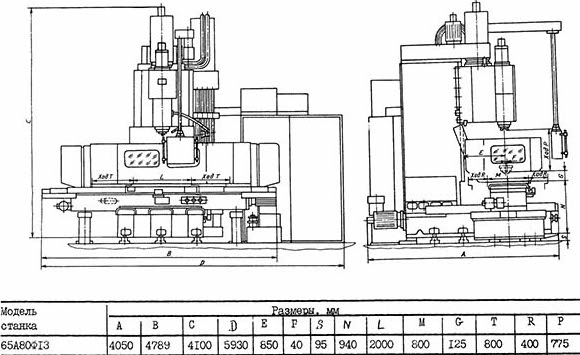
\includegraphics[width=.90\linewidth]{spr_65a80_1.jpg}
    \caption{габаритные размеры рабочего поля}
    \label{subfig:65a80a}
  \end{subfigure}%
  \begin{subfigure}[b]{.50\textwidth}
    \centering
    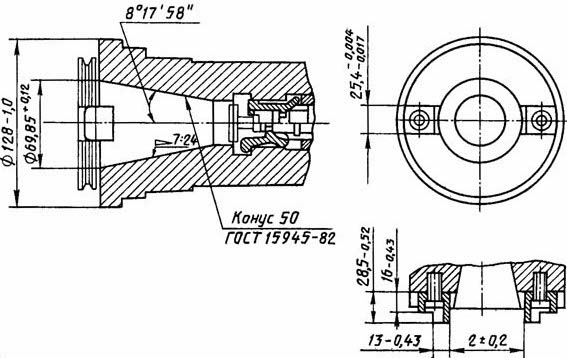
\includegraphics[width=.90\linewidth]{spr_2206vmf4_2.jpg}
    \caption{посадочные и присоединительные базы}
    \label{subfig:65a80b}
  \end{subfigure}%
  \caption{Посадочные и присоединительные размеры станка 65А80}
  \label{fig:65a80}
\end{figure}

\newpage
\subsection{Выбор и обоснование схемы базирования}

Базирование осуществляется по схеме, представленной на рис.~\ref{fig:b045}

\begin{figure}[H]
	\centering
	   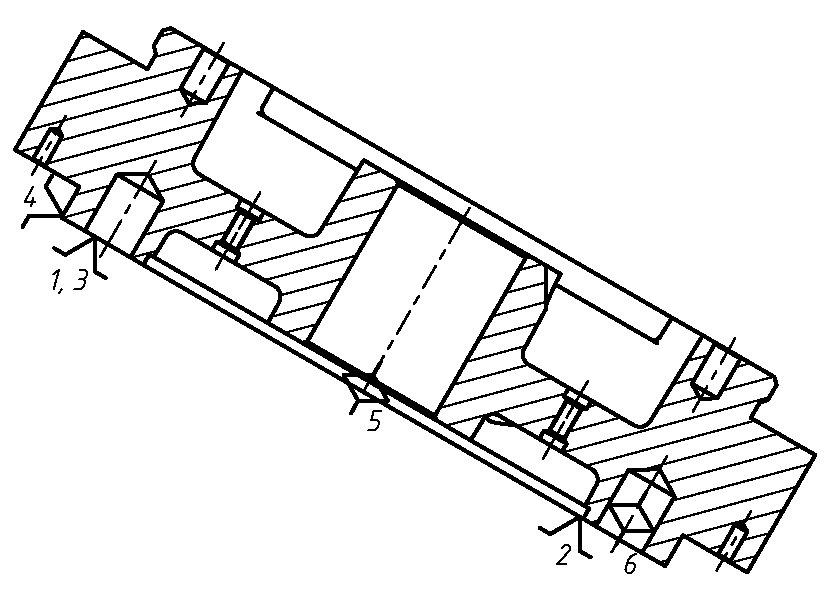
\includegraphics[width=0.7\textwidth]{bases_045.pdf}
	   \caption{Схема базирования на операции 045}
	   \label{fig:b045}
	   1, 2, 3 --- установочная база, \\
	   4, 5 --- направляющая база, \\
	   6 --- опорная база
\end{figure}

\subsection{Выбор и обоснование последовательности и содержания переходов}

На операции 045 осуществляется обработка паза, расположенных под углом к торцу детали. Деталь установлена в специальном приспособлении под наклоном. Обработка паза производится за один проход концевой фрезой, радиус которой совпадает с радиусом скруглений паза. Последовательность обработки приведена в табл.~\ref{tab:045}

\begin{table}[H]
  \setlength{\tabulinesep}{1.2ex}
  \begin{longtabu} to \textwidth { | X[7,l,p] | }
    \caption{Содержание основных переходов операции 045} \label{tab:045} \\
  
      \hline 
      \multicolumn{1}{|c|}{\linespread{1.1} \bfseries{\small Содержание переходов}} \\ \hline 
    \endfirsthead
  
      \multicolumn{1}{l}{{\itshape Продолжение таблицы \thetable{}}} \\ \hline 
      \multicolumn{1}{|c|}{\linespread{1.1} \bfseries{\small Содержание переходов}} \\ \hline
    \endhead
  
      \hline
    \endfoot

      -- Фрезеровать паз \circled{34}, выдерживая размер $20 \times \ang{60}$ и ширину $50$ \\ \hline

  \end{longtabu}
\end{table}

\subsection{Выбор и характеристика режущего инструмента}




\subsection{Расчёт режимов и сил резания}
\subsection{Техническое нормирование}
\subsection{Выбор методов и средств операционного контроля}


\chapter{Расчёт и проектирование станочных приспособлений}

\section{Приспособление для расточной операции с ЧПУ}

\subsection{Характеристика и описание принципа работы приспособления}
\subsection{Силовой расчёт приспособления}
\subsection{Прочностной расчёт приспособления}
\subsection{Точностной расчёт приспособления}

\section{Приспособление для фрезерной операции}

\subsection{Характеристика и описание принципа работы приспособления}
\subsection{Силовой расчёт приспособления}
\subsection{Прочностной расчёт приспособления}
\subsection{Точностной расчёт приспособления}


\likechapter{Список использованных источников}

\nocite{malvyat:okp}

\nocite{burtsev:tm2}
\nocite{bezyazichny:otm}
\nocite{blumenstejn:pto}
\nocite{kosilova:stm2}
\nocite{tarabarin:pto}
\nocite{gost:2-121-73}
\nocite{gost:14-205-83}
\nocite{gost:3-1404-86}
\nocite{gost:3-1118-88}
\nocite{gost:2-105-95}
\nocite{gost:3-1702-79}

\printbibliography[heading=none]


\end{document}